\subsection{Secant Method}
One disadvantage of Newton's Method is that evaluating $f^{\prime}(x)$ can be costly or difficult. This motivates the \textbf{secant method}, which instead approximates $f^{\prime}$ using a \textbf{secant line} between $f(x_k)$ and $f(x_{k-1})$.
\[f\left[x_{k-1}, x_k\right]=\frac{f\left(x_k\right)-f\left(x_{k-1}\right)}{x_k-x_{k-1}}\]
The basic idea is to pick $x_0$ and $x_1$ and then iteratively define,
\[x_{k+1}=x_k-\frac{f\left(x_k\right)}{f\left[x_{k-1}, x_k\right]}\]

\begin{marginfigure}
\begin{center}
       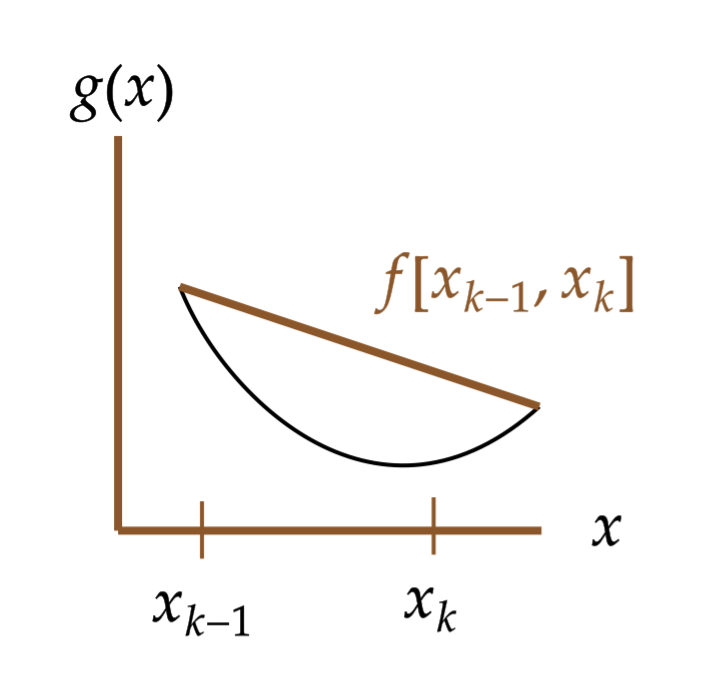
\includegraphics[width=0.8\textwidth]{figures/fig-3.png}
\end{center}
\end{marginfigure}

\begin{marginfigure}
    In order to converge, the Secant Method requires two initial guesses $x_0$ and $x_1$ which are sufficiently close to $x^*$.
\end{marginfigure}

\begin{defn}[Lagrange Interpolation Error]
   \sloppy Let $f \in C^2[a, b]$ and $z_0, z_1 \in [a, b]$. There exists $\xi(x)$ between $z_0, z_1$ such that,
   \[
    f(x)=\underbrace{f\left(z_0\right)+f\left[z_1, z_0\right]\left(x-z_0\right)}_{f_1(x)}+\underbrace{\frac{f^{\prime \prime}(\xi(x))}{2 !}\left(x-z_0\right)\left(x-z_1\right)}_{R_1(x)}
    \]
    for all $x \in [a,b]$.
\end{defn}

\begin{rmk}
\sloppy The Lagrange Interpolation Error is analogous to Taylor's Theorem with the derivative replaced by the secant. $f_1(x)$ represents $P_1(x)$ and $R_1(x)$ represents the remainder term.
\end{rmk}

\begin{thm}
   The secant method converges superlinearly, but slower than quadratic. Its convergence order is equal to the \textbf{golden ratio}.
\end{thm}

\begin{proof}
   We can re-write the secant method at the $k$-th iteration as,
   \[
    0=f\left(x_k\right)+f\left[x_{k-1}, x_k\right]\left(x_{k+1}-x_k\right)
    \]
   By the Mean Value Theorem, there exists $\eta_k$ such that,
    \[0 = f\left(x_k\right)+f^{\prime}\left(\eta_k\right)\left(x_{k+1}-x_k\right)\]
   By definition of the Lagrange Interpolation Error with,
   \[z_0=x_k \quad \quad z_1=x_{k-1} \quad \quad x=x^*\]
   we obtain the following,
   \[0=f\left(x_k\right)+f\left[x_{k-1}, x_k\right]\left(x^*-x_k\right)+\frac{f^{\prime \prime}\left(\xi\left(x^*\right)\right)}{2}\left(x^*-x_k\right)\left(x^*-x_{k-1}\right)\]
Subtracting the two equations gives that,
\[x^*-x_{k+1}=A_k\left(x^*-x_k\right)\left(x^*-x_{k-1}\right) \text{ where } A_k = \frac{f^{\prime \prime}\left(\xi\left(x^*\right)\right)}{2 f^{\prime}\left(\eta_k\right)}\]
If a sequence $\{x_k\}_k$ converges to $x^*$ at order $p$, then for large $k$ there exist constants $C_1, C_2 > 0$ and $r \in (0, 1)$ such that,
\[C_1 r^{p^k} \leq\left|x^*-x_k\right| \leq C_2 r^{p^k}\]
Consequently,
\begin{align*}
C_1 r^{p^{k+1}} &\leq\left|x^*-x_{k+1}\right| \\
&=\left|A_k\right|\left|x^*-x_k\right|\left|x^*-x_{k-1}\right| \\
&\leq\left|A_k\right|\left(C_2 r^{p^k}\right)\left(C_2 r^{p^{k-1}}\right)
\end{align*}
Moreover,
\begin{align*}
    \left|A_k\right|\left(C_1 r^{p^k}\right)\left(C_1 r^{p^{k-1}}\right) &\leq\left|A_k\right|\left|x^*-x_k\right|\left|x^*-x_{k-1}\right| \\
    &=\left|x^*-x_{k+1}\right| \leq C_2 r^{p^{k+1}}
\end{align*}
Re-arranging gives that,
\[0<\frac{C_1}{\left|A_k\right| C_2^2} \leq r^{p^k+p^{k-1}-p^{k+1}} \leq \frac{C_2}{\left|A_k\right| C_1^2} \text{ where } \left|A_k\right| \rightarrow \frac{\left|f^{\prime \prime}\left(x^*\right)\right|}{2\left|f^{\prime}\left(x^*\right)\right|}\]
since $r \in (0, 1)$, these inequalities require that,
\[0=p^k+p^{k-1}-p^{k+1}=p^{k-1}\left(p+1-p^2\right)\]
Solving gives the golden ratio,
\[p=\frac{1+\sqrt{5}}{2} \approx 1.61803 \ldots\]
\end{proof}

\subsection{Summary}
We saw the following numerical methods,
\begin{table}[h]
\begin{tabularx}{\textwidth}{lll}
\toprule
\textbf{Method} & \textbf{Convergence Criteria} & \textbf{Order} \\
\midrule
Bisection & $f \in C[a, b]$ and $x_0 \in[a, b]$ & Linear \\
\midrule
Fixed Point
&- Fixed Point Theorem (1) &  \\
&- Fixed Point Theorem (2) & Linear \\
&- $g^{\prime}\left(x^*\right) \neq 0$ &  \\
\midrule
Newton
&- $f^{\prime}\left(x^*\right) \neq 0$ & \\
&- $f^{\prime\prime}\left(x^*\right) \neq 0$ & Quadratic \\
&- $x_0$ close to $x^*$ & \\
\midrule
Secant
&- $f^{\prime}\left(x^*\right) \neq 0$ & \\
&- $f^{\prime\prime}\left(x^*\right) \neq 0$ & Golden Ratio \\
&- $x_0$ close to $x^*$ & \\
\bottomrule
\end{tabularx}
\end{table}